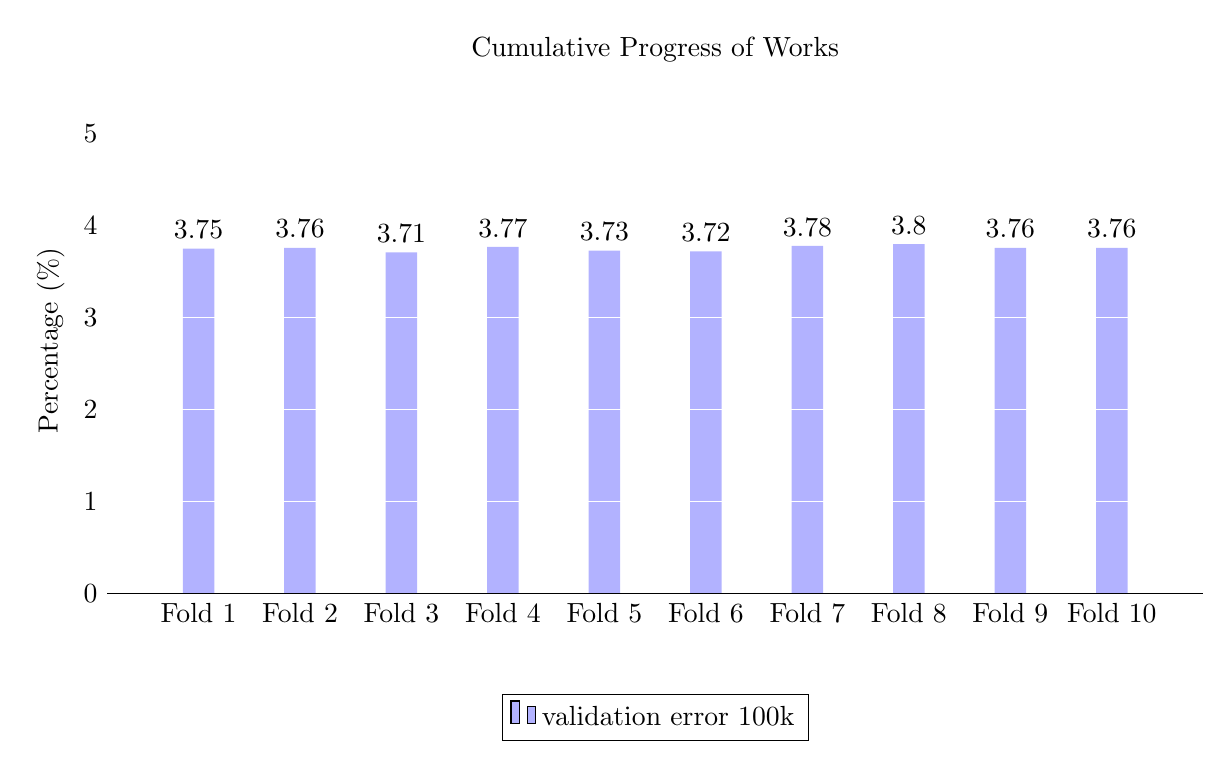
\begin{tikzpicture}
  \centering
  \begin{axis}[
        ybar, axis on top,
        title={Cumulative Progress of Works},
        height=8cm, width=15.5cm,
        bar width=0.4cm,
        ymajorgrids, tick align=inside,
        major grid style={draw=white},
        enlarge y limits={value=.1,upper},
        ymin=0, ymax=5,
        axis x line*=bottom,
        y axis line style={opacity=0},
        tickwidth=0pt,
        enlarge x limits=true,
        legend style={
            at={(0.5,-0.2)},
            anchor=north,
            legend columns=-1,
            /tikz/every even column/.append style={column sep=0.5cm}
        },
        ylabel={Percentage (\%)},
        symbolic x coords={
           Fold 1,Fold 2,
           Fold 3,Fold 4,
           Fold 5,Fold 6,
           Fold 7,Fold 8,
           Fold 9,Fold 10},
       xtick=data,
       nodes near coords={
        \pgfmathprintnumber[precision=2]{\pgfplotspointmeta}
       }
    ]
    \addplot [draw=none, fill=blue!30] coordinates {
      (Fold 1, 3.75)
      (Fold 2, 3.76)
      (Fold 3, 3.71)
      (Fold 4, 3.77)
      (Fold 5, 3.73)
      (Fold 6, 3.72)
      (Fold 7, 3.78)
      (Fold 8, 3.80)
      (Fold 9, 3.76)
      (Fold 10, 3.76)};
%   \addplot [draw=none,fill=red!30] coordinates {
%      (Fold 1, 3.75)
%      (Fold 2, 3.76)
%      (Fold 3, 3.71)
%      (Fold 4, 3.77)
%      (Fold 5, 3.73)
%      (Fold 6, 3.72)
%      (Fold 7, 3.78)
%      (Fold 8, 3.80)
%      (Fold 9, 3.76)
%      (Fold 10, 3.76)};
%   \addplot [draw=none, fill=green!30] coordinates {
%      (Sep-11,75.4064)
%      (Oct-11, 89.7961) 
%      (Nov-11,94.4597)
%      (Dec-11,76.6786) 
%      (Jan-12,77.5600) 
%      (Feb-12,78.2339)
%      (Mar-12,88.6138) 
%      (Apr-12,78.9129) };

    \legend{validation error 100k, test error 100k}
  \end{axis}
  \end{tikzpicture}